\documentclass[./00PhotoBox.tex]{subfiles}
\graphicspath{{\subfix{./img/}}}
\begin{document}


\chapter{Aufbau des Messsystemes}
Die Kameras sollten eine hohe geometrische Auflösung und möglichst stabile innere Orientierung aufweisen. Außerdem sollen sie während einer Messkampagne nicht in ihrer Lage zueinander verändert werden, damit die äußere Orientierung größtenteils unverändert bleibt. Daher ist ein stabiler Rahmen notwendig, an welchem die Kameras verdrehsicher angebracht werden können. Kleinere Restfehler in den Orientierungen können mit ausgeglichen werden.
Um Ungenauigkeiten durch Bewegungen zu verhindern, müssen die Kameras möglichst zeitgleich auslösen. Daher ist eine gemeinsame Steuerung und Kommunikation zwischen den Kameras notwendig. Außerdem sollen alle Bilder dann auf das Steuerungssystem übertragen werden, hierfür wir eine Form der Datenübertragung benötigt. Damit die Bilder möglichst schattenfrei ausgeleuchtet werden, muss Beleuchtung mit eingeplant werden. Außerdem muss die Stromversorgung der einzelnen Kameras sichergestellt sein.

Aus diesen Anforderungen ergeben sich die einzelnen Abschnitte dieses Kapitels.

\section{Kameras}
Als Kameras wurde das Raspberry Pi Camera Module 3 verwendet, welches jeweils von einem Raspberry Pi Zero W gesteuert wird. Im Vergleich zu anderen günstigen Kameras wie Webcams oder der ESP32 CAM haben die Kameras eine hohe geometrische Auflösung von 12 Megapixeln und dennoch mit $1,4~\mu m$ relativ große Pixel \citep{raspicamdatasheet}, was im subjektiven Eindruck eine sehr gute Bildqualität ergibt.

Andere Kameramodule für den Raspberry Pi wurden in \autoref{tab:vergleich_kameras} verglichen. Das Camera Module v1 entfiel als Möglichkeit, da die Kamera einen Mindestabstand von einem Meter aufwies. Hiermit müsste der Aufnahmebereich für die Objekte auf über zwei Meter vergrößert werden. Die HQ- und GS-Kameras haben kein Objektiv mitgeliefert, sodass hier die Kosten für ein Objektiv hinzukommen würden. Das Camera Module v2 hat eine geringere Auflösung und auch eine geringere Bildqualität bei gleichem Preis wie das Modul v3. Außerdem ist die Fokussierung nur manuell möglich, dass die Automatisierung desselben verhindert. Das Camera Module v3 Wide hat zwar ein größeres Sichtfeld, jedoch damit auch eine geringere Auflösung auf dem Objekt. Vorteil ist der geringe Mindestabstand. Da das Camera Module v3 besser verfügbar war, etwas günstiger war und damit einen guten Kompromiss bildete, wurde sich für dieses Modell entschieden.

\begin{table}
    \centering
    \caption{Vergleich der möglichen Kameramodule für den Raspberry Pi \citep{raspicamdatasheet}}
    \label{tab:vergleich_kameras}
    \resizebox{\textwidth}{!}{%
        \begin{tabular}{l|l|l|l|ll|l|l|l|}
            \cline{2-9}
                                                                & \textbf{Preis}               & \textbf{\begin{tabular}[c]{@{}l@{}}Sensor-\\ auflösung\end{tabular}} & \textbf{\begin{tabular}[c]{@{}l@{}}Pixel\\ {[}µm{]}\end{tabular}} & \multicolumn{2}{l|}{\textbf{Fokus}}                                         & \textbf{f {[}mm{]}}                                           & \textbf{Sichtfeld}       & \textbf{Blende}                                         \\ \hline
            \multicolumn{1}{|l|}{\textbf{Camera Module v1}}     & \$25                         & 2592 × 1944                                                          & 1,40                                                              & \multicolumn{1}{l|}{\cellcolor[HTML]{FFCCC9}fix}                            & \cellcolor[HTML]{FFCCC9}{\color[HTML]{000000} 1 m - $\infty$} & 3,60                     & 54° x 41°                & F2.9                         \\ \hline
            \multicolumn{1}{|l|}{\textbf{Camera Module v2}}     & \$25                         & 3280 × 2464                                                          & 1,12                                                              & \multicolumn{1}{l|}{\cellcolor[HTML]{FFCCC9}manuell}                        & 10 cm - $\infty$                                              & 3,04                     & 62° x 49°                & F2.0                         \\ \hline
            \multicolumn{1}{|l|}{\textbf{Camera Module 3}}      & \cellcolor[HTML]{9AFF99}\$25 & \cellcolor[HTML]{9AFF99}4608 x 2592                                  & 1,40                                                              & \multicolumn{1}{l|}{\cellcolor[HTML]{9AFF99}motorisiert}                    & 10 cm - $\infty$                                              & 4,74                     & 66° x 41°                & \cellcolor[HTML]{9AFF99}F1.8 \\ \hline
            \multicolumn{1}{|l|}{\textbf{Camera Module 3 Wide}} & \$35                         & \cellcolor[HTML]{9AFF99}4608 x 2592                                  & 1,40                                                              & \multicolumn{1}{l|}{\cellcolor[HTML]{9AFF99}motorisiert}                    & \cellcolor[HTML]{9AFF99}5 cm - $\infty$                       & 2,75                     & 102° x 67°               & F2.2                         \\ \hline
            \multicolumn{1}{|l|}{\textbf{HQ Camera}}            & \cellcolor[HTML]{FFCCC9}\$50 & 4056 x 3040                                                          & 1,55                                                              & \multicolumn{1}{l|}{\cellcolor[HTML]{FFCCC9}{\color[HTML]{000000} manuell}} & \cellcolor[HTML]{C0C0C0}                                      & \cellcolor[HTML]{C0C0C0} & \cellcolor[HTML]{C0C0C0} & \cellcolor[HTML]{C0C0C0}     \\ \hline
            \multicolumn{1}{|l|}{\textbf{GS Camera}}            & \cellcolor[HTML]{FFCCC9}\$50 & 1456 x 1088                                                          & \cellcolor[HTML]{9AFF99}3,45                                      & \multicolumn{1}{l|}{\cellcolor[HTML]{FFCCC9}{\color[HTML]{000000} manuell}} & \cellcolor[HTML]{C0C0C0}                                      & \cellcolor[HTML]{C0C0C0} & \cellcolor[HTML]{C0C0C0} & \cellcolor[HTML]{C0C0C0}     \\ \hline
        \end{tabular}
    }
\end{table}

Nachteil und Vorteil zugleich ist, dass die Kamera über einen Autofokus verfügt, der aber auch elektronisch gesteuert manuell fokussieren kann. Dieser verschlechtert die Stabilität der inneren Orientierung (vgl. \autoref{s:innereorientierung}) weiter und wurde daher auch besonders im \autoref{c:voruntersuchungen} analysiert. Da die Bilder im Makrobereich zwischen $10$ und $80~\text{cm}$ aufgenommen werden und die Kameras keine Veränderung der Blende ermöglichen, ist die Schärfentiefe vergleichsweise niedrig. Hierauf wird in den Untersuchungen in \autoref{sec:fokusstacking} speziell eingegangen.

Weiterer Vorteil der Lösung mit einzelnen Raspberry Pi ist es, dass hierdurch bereits die einzelnen Kameraeinheiten Berechnungen wie das Identifizieren von Passpunkten übernehmen können. Durch die Parallelisierung dieses Schrittes ist weniger Berechnungszeit zwischen den Aufnahmen zu erwarten. Außerdem ist durch die Nutzung von kabellosen Netzwerkverbindungen zur Steuerung das System skalierbar im Sinne der Anzahl der Kameras aber auch der Abstände zwischen den Kameras.

\todo{virtuelles Blendermodell}



\section{Rahmen}

\begin{figure}
    \centering
    \begin{subfigure}{0.45\textwidth}
        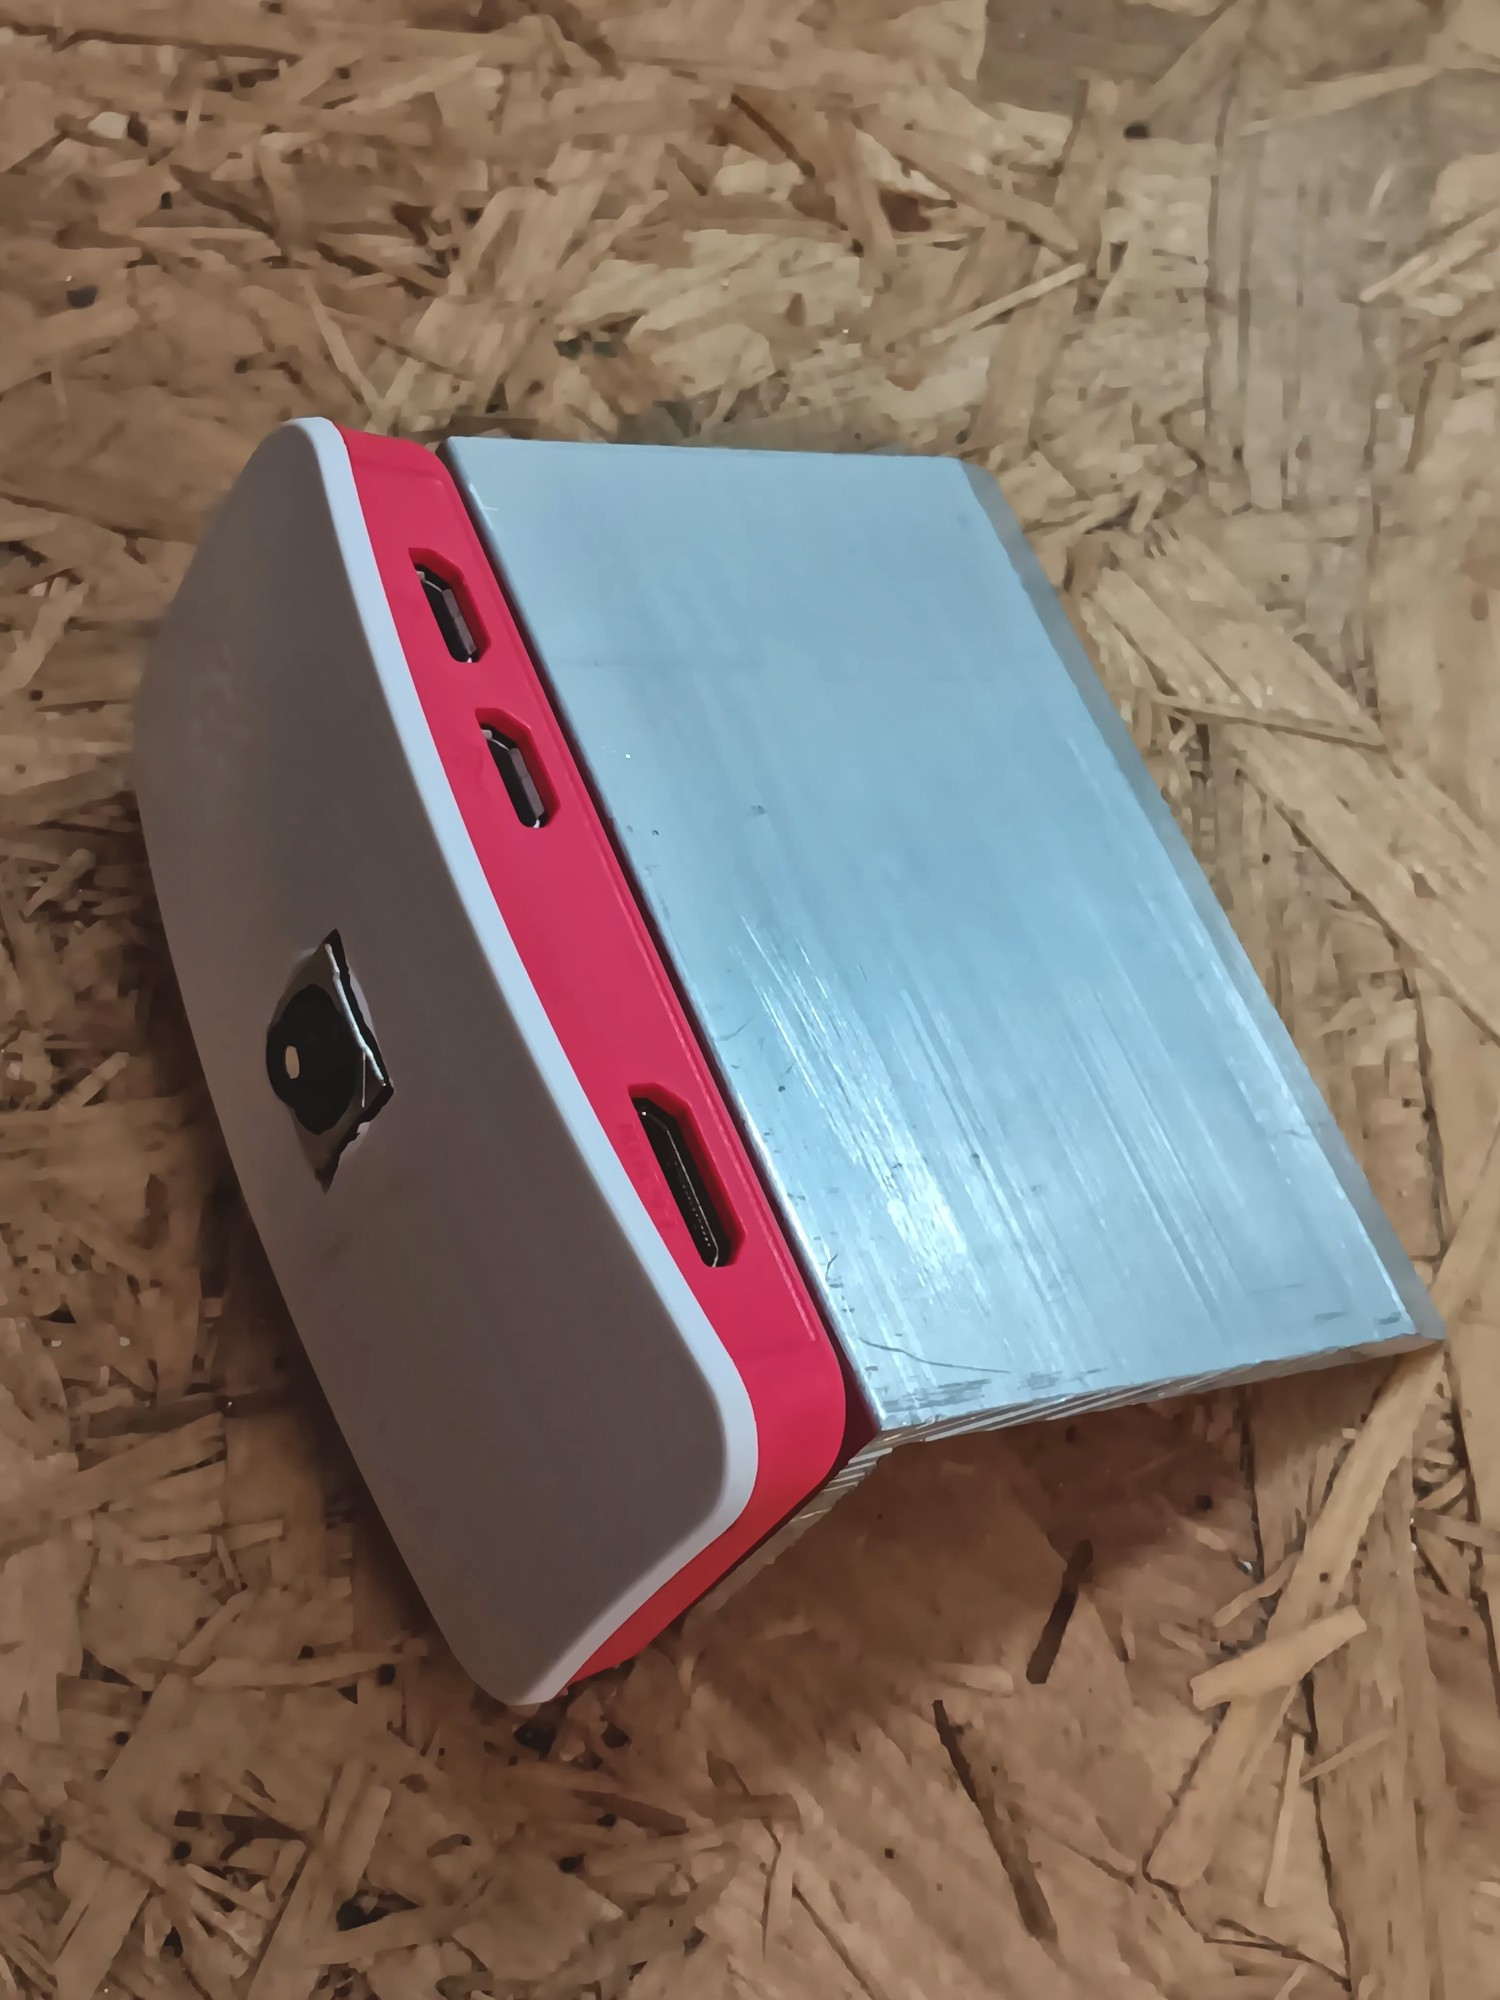
\includegraphics[height=0.9\linewidth]{./img/aluwinkel.jpg}
        \centering
        \caption{Kamera-Winkel} %Bildunterschrift
        \label{img:aluwinkel} %ID fürs Bild
    \end{subfigure}
    \begin{subfigure}{0.45\textwidth}
        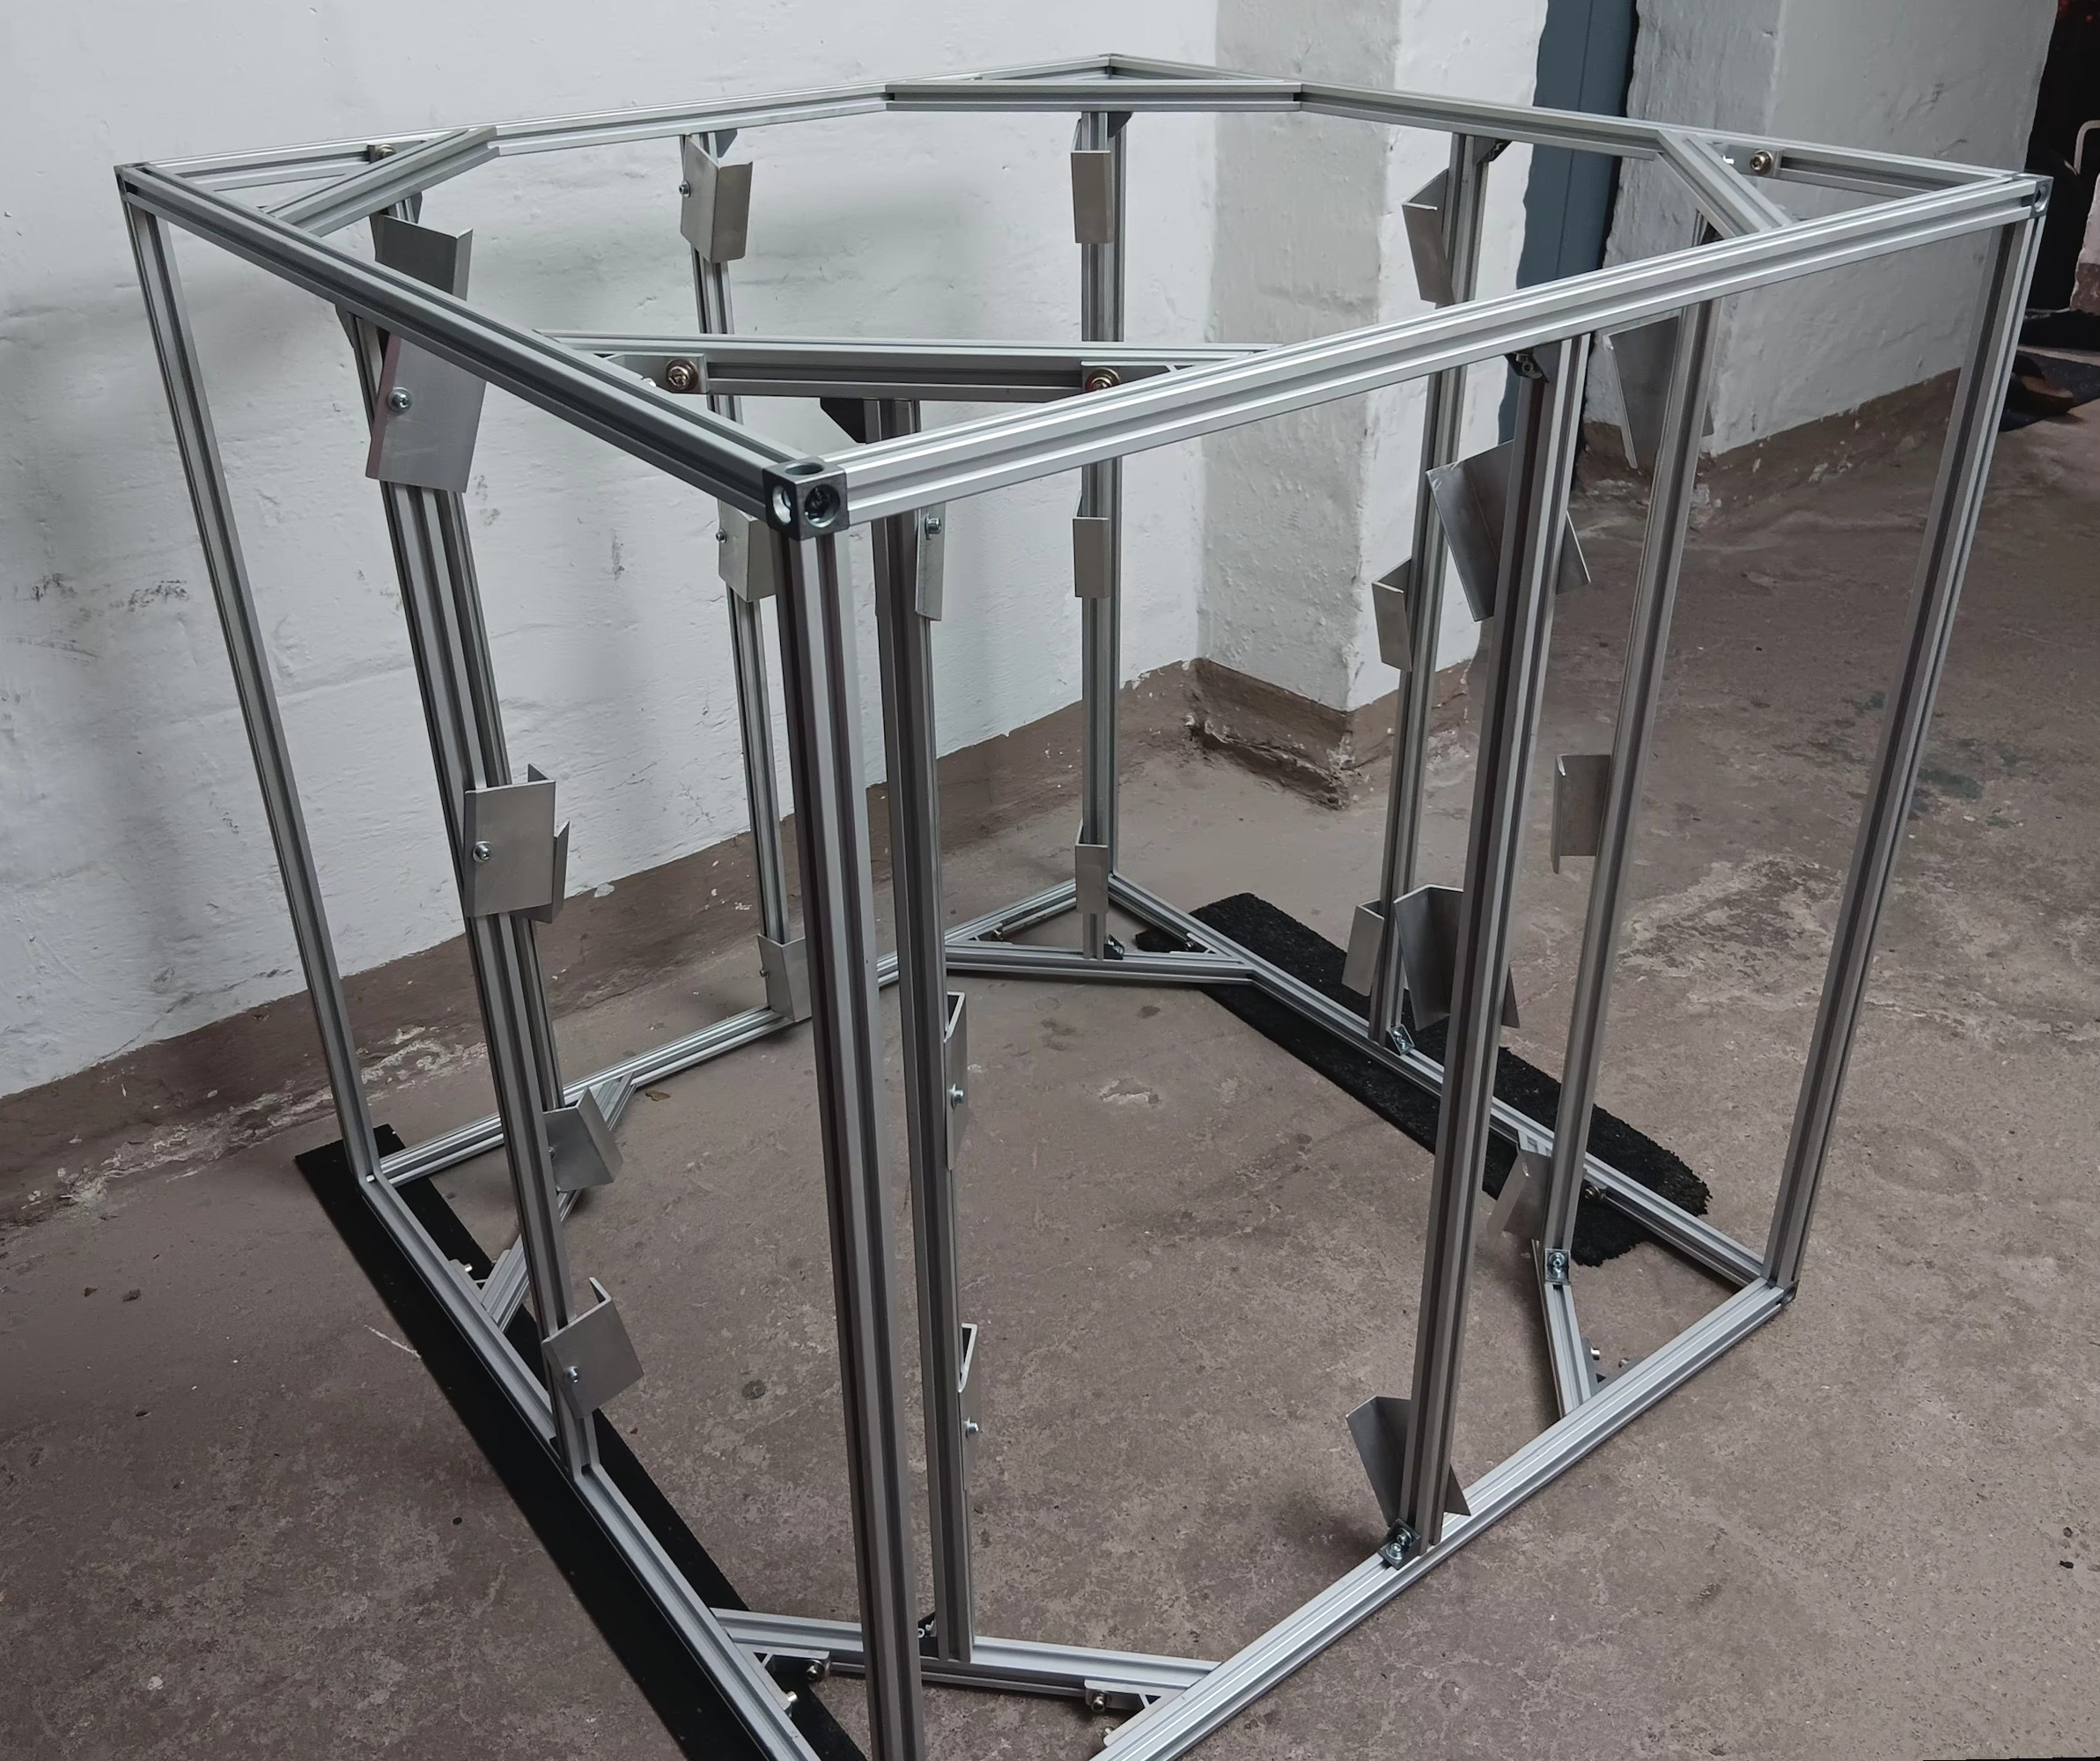
\includegraphics[height=0.8\linewidth]{./img/alurahmen.jpg}
        \centering
        \caption{Aluminium-Rahmen} %Bildunterschrift
        \label{img:alurahmen} %ID fürs Bder an den Aluprofilen befestigt ist (ild
    \end{subfigure}
    \caption{Rahmen und Kameramontage-Winkel} %Bildunterschrift
\end{figure}

Der Rahmen muss möglichst stabil sein, damit die Kameras sich nicht in ihrer Lage verändern können. Jedoch sollte das System auch weiterhin transportabel - also nicht zu schwer - und veränderbar bleiben, beispielsweise Kameras für Messreihen in ihrer Lage verändert werden. Der Aufbau aus genormten Bauteilen bietet sich an, um hier ggf. den Nachbau einfach ermöglichen zu können. Außerdem sollte der Rahmen auch gegebenenfalls demontierbar sein, damit er transportiert werden kann.

Als mögliche Materialien kamen Holz, Stahl und Aluminium infrage. Aufgrund der einfachen Bearbeitung und der genormten Profile wurde sich für Aluminiumprofile entschieden. Diese gibt es in verschiedenen Ausführungen mit Nuten an den Seitenflächen, sodass eine einfache Montage, aber auch eine Demontage zu Transportzwecken, möglich wird. Außerdem sind diese sehr stabil bei leichtem Gewicht. Durch eine Konstruktion mit Eckwürfeln sowie dem Einbau von dreieckigen Strukturen und Platten, die Scheibenwirkung haben, wurde die Stabilität der Verbindungen erhöht. \autoref{img:alurahmen} zeigt den fertigen Rahmen vor Einbau der Platten und der Technik.

Die Kameras wurden mit einem $90^\circ$-Winkel am Rahmen montiert, um diese weiterhin noch vertikal schwenken zu können. \autoref{img:aluwinkel} zeigt einen der Winkel, der an den Aluprofilen befestigt ist (noch ohne entsprechende Befestigungsbohrungen).


\section{Beleuchtung}


\begin{figure}
    \centering
    \begin{subfigure}{0.45\textwidth}
        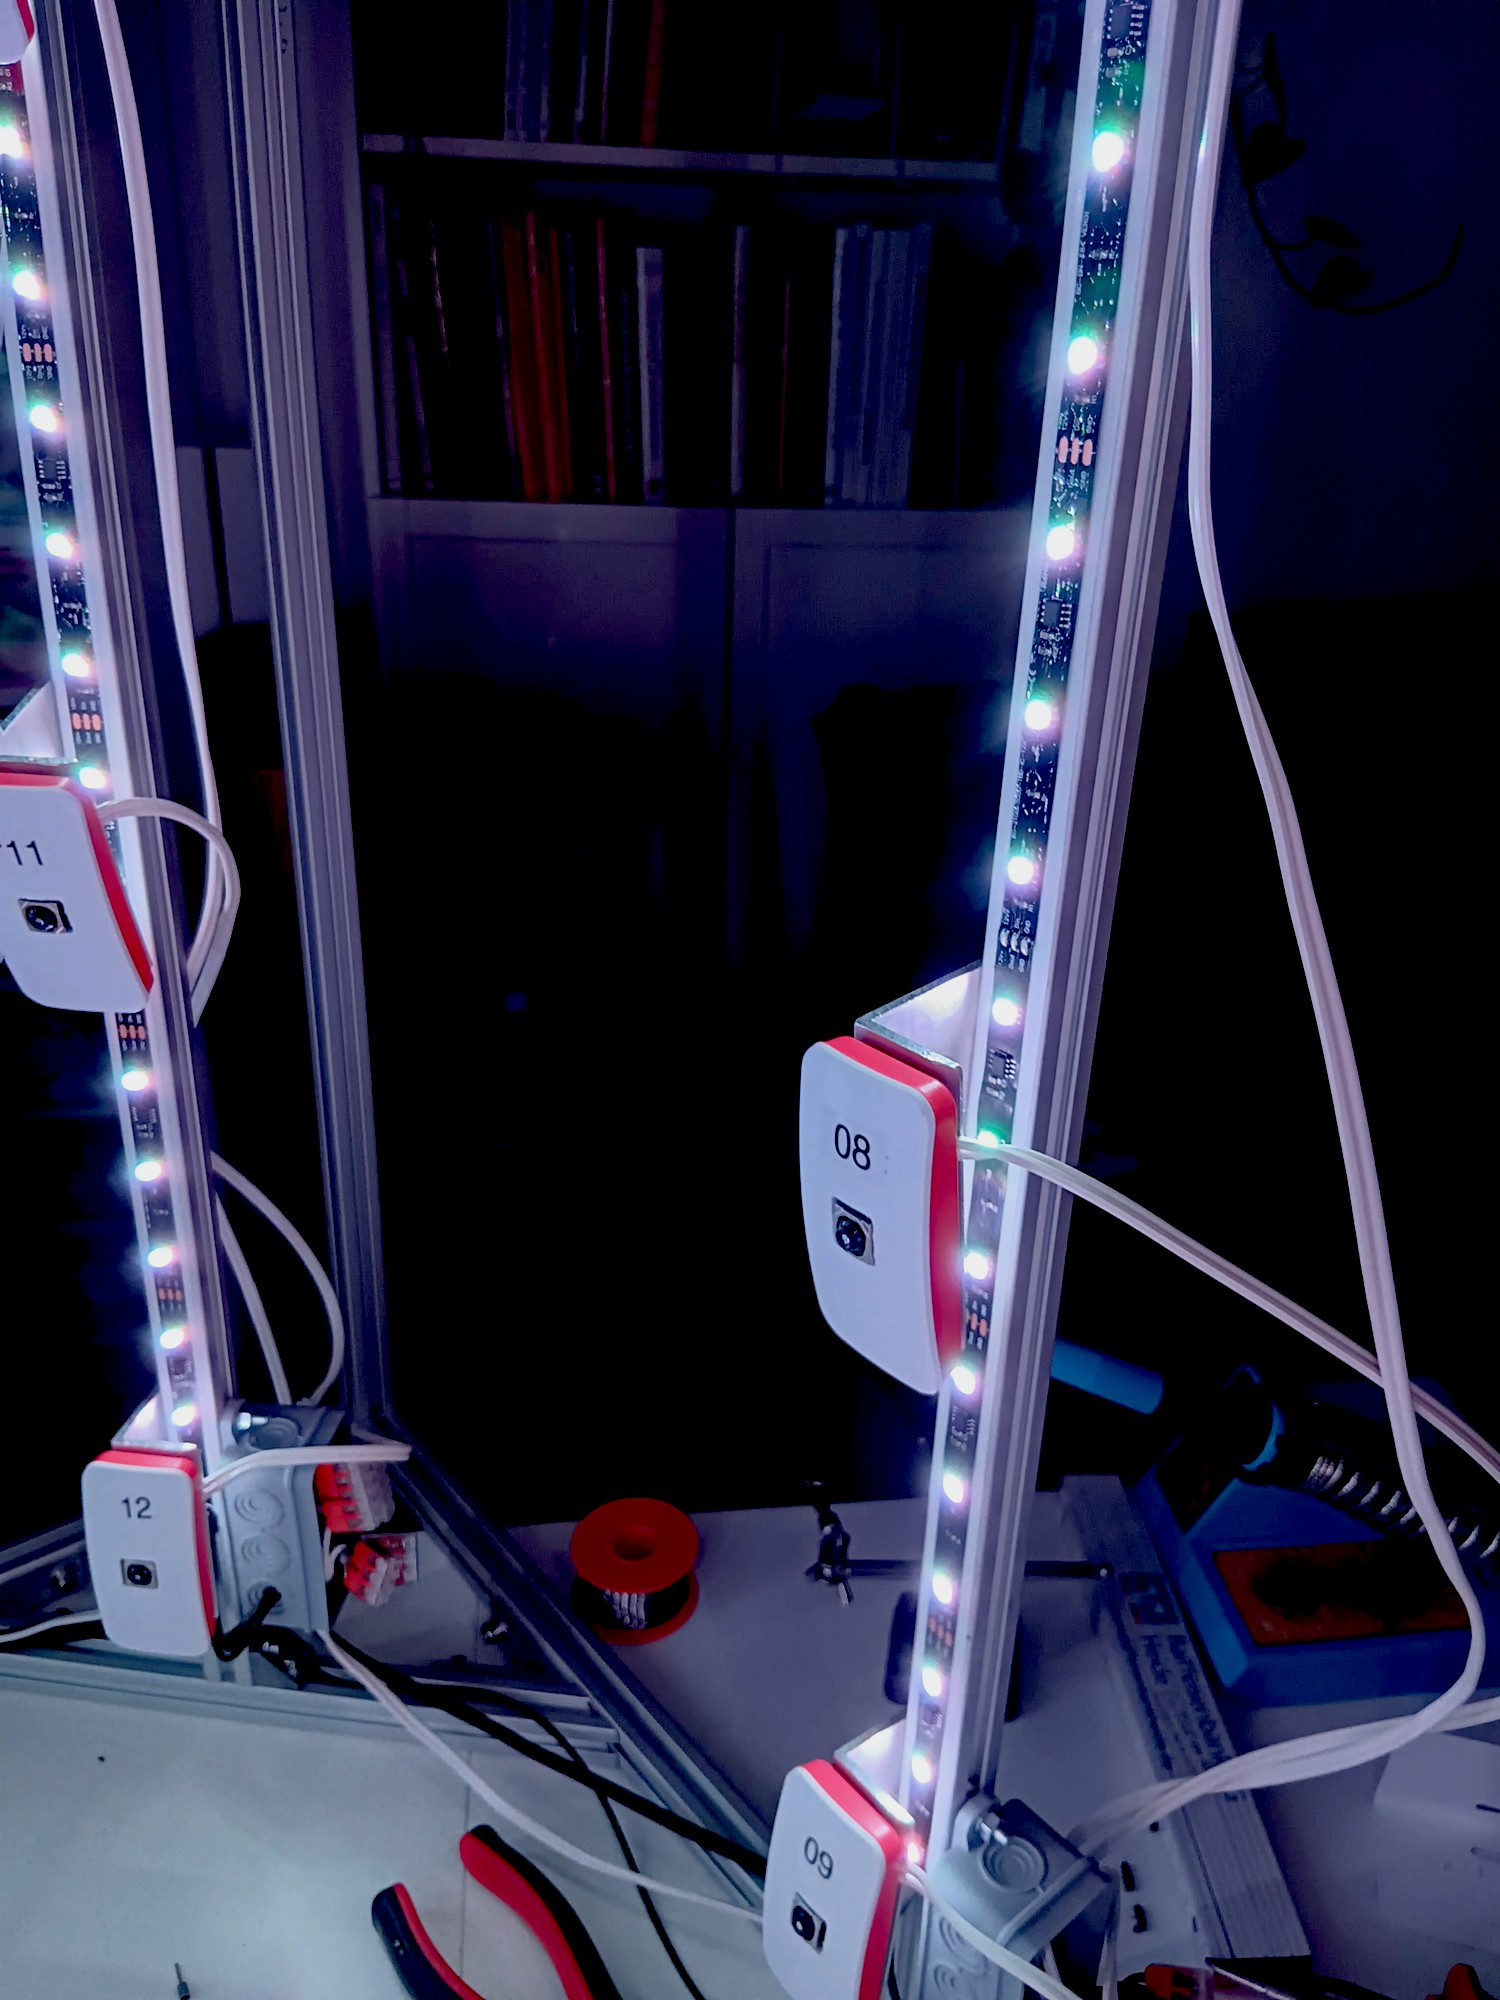
\includegraphics[height=1.2\linewidth]{./img/beleuchtung.jpg}
        \centering
        \caption{Schattenarme Beleuchtung durch LED-Streifen}
        \label{img:led_streifen}
    \end{subfigure}
    \begin{subfigure}{0.45\textwidth}
        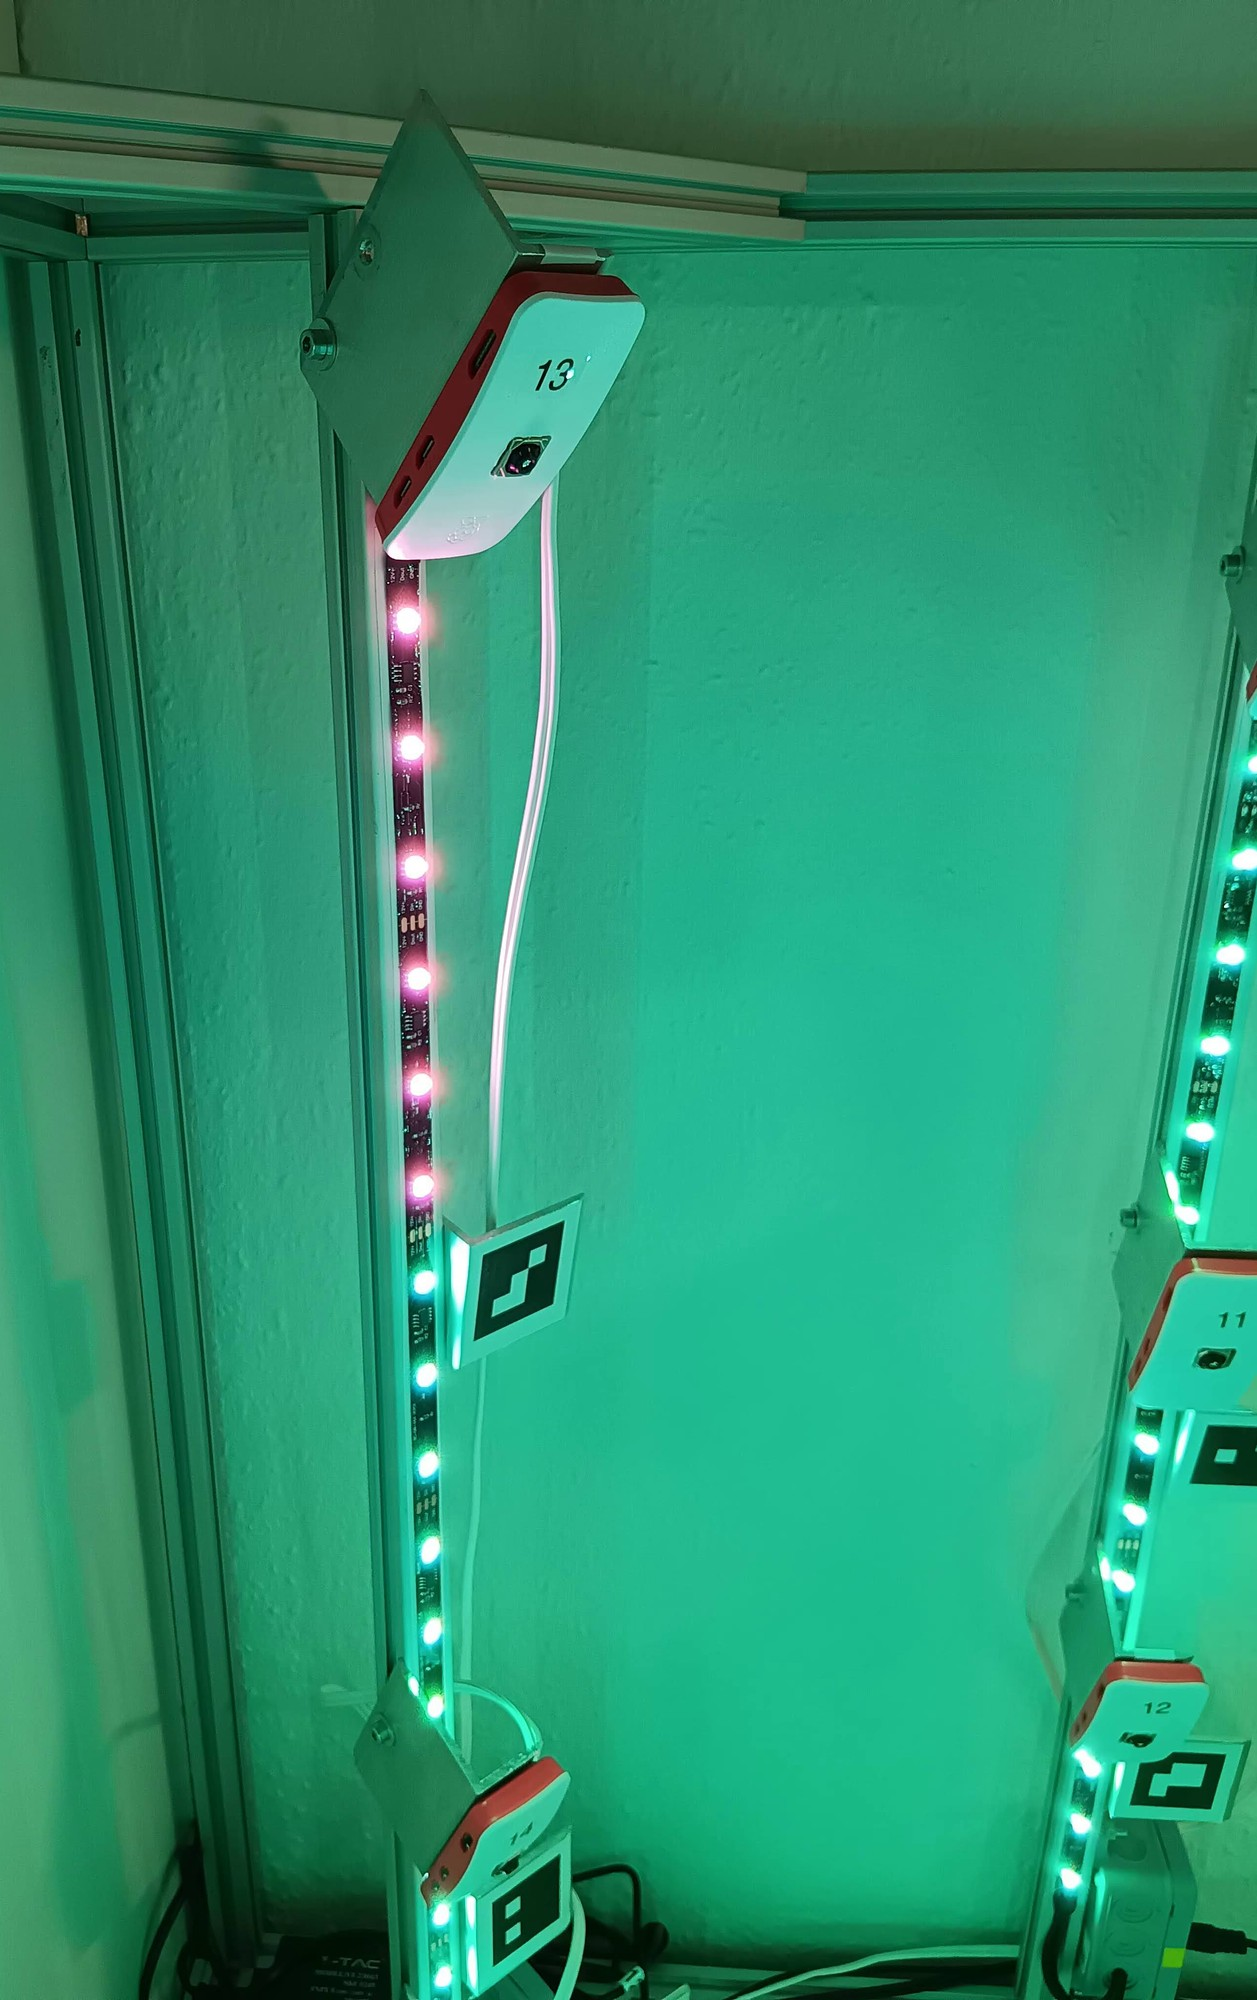
\includegraphics[height=1.2\linewidth]{./img/beleuchtung_farbig.jpg}
        \centering
        \caption{Farbige Beleuchtung zur Statusmeldung}
        \label{img:led_farbig}
    \end{subfigure}
    \caption{Beleuchtung}
\end{figure}

Um möglichst gute Bilder zu erzeugen, sollte das Objekt ausreichend und gleichmäßig ausgeleuchtet sein. Eine dunkle Umgebung verlängert die Belichtungszeit, wodurch die Gefahr von unscharfen Aufnahmen steigt. Schlecht ausgeleuchtete Bereiche (ungleichmäßige Ausleuchtung) verursachen verstärktes Rauschen in diesen Bildbereichen. Daher soll das System eine gleichmäßige Ausleuchtung ermöglichen. Problematisch ist hierbei, dass die Kameras ggf. auch die Lichtquellen mit im Bildbereich haben können, wodurch Linsenreflexionen oder Ausbrennen der Bildbereiche möglich sind. Außerdem störend sind fremde Lichtquellen, die Schatten werfen oder die Belichtung der Kameras beeinflussen können.

Es wurde sich zur Beleuchtung für einzeln steuerbare LED-Lichtstreifen entschieden (siehe \autoref{img:led_streifen}). Diese können einfach an den Aluprofilen montiert werden und ermöglichen es, einzelne Bereiche und so ggf. blendende Bereiche abzuschalten. Außerdem können hiermit auch verschiedene Lichtfarben eingestellt werden, um Statusmeldungen zu geben (siehe \autoref{img:led_farbig}) oder ggf. die Farbgebung des Objektes zu beeinflussen. Die Steuerung erfolgt über einen Raspberry Pi 4, der auch die Steuerung der Kameras übernimmt. Die LED-Streifen verfügen hierfür pro drei LEDs über einen integrierten Schaltkreis vom Typ WS2811. Dieser ermöglicht es, jeden Dreier-Verbund über ein proprietäres Steuerprotokoll eine eigene Farbe und Helligkeit zuzuweisen \citep{ws2811}. Für die Implementierung der Steuerung wurde die Bibliothek \texttt{rpi-ws281x} verwendet, die eine einfache Ansteuerung der LED-Streifen ermöglicht (siehe auch \autoref{p:ws281x}).

Für diffuseres Licht von außen kann ein halbtransparenter, weißer Stoff über den Rahmen gespannt werden. Dieser sorgt für eine gleichmäßigere Ausleuchtung durch Reflexion im Inneren, verhindert auch Reflexionen an Glasscheiben und ähnlichem und vermindert Blendwirkungen durch externe Lichtquellen. Hierfür wurde aus weißem Baumwollstoff eine entsprechende Haube genäht, welche durch zwei mittels Reißverschluss verschließbaren Eingriffmöglichkeiten weiterhin das Einlegen von Objekten durch die Seite oder das Verstellen von Kameras ermöglicht.


\section{Stromversorgung}

\begin{figure}
    \centering
    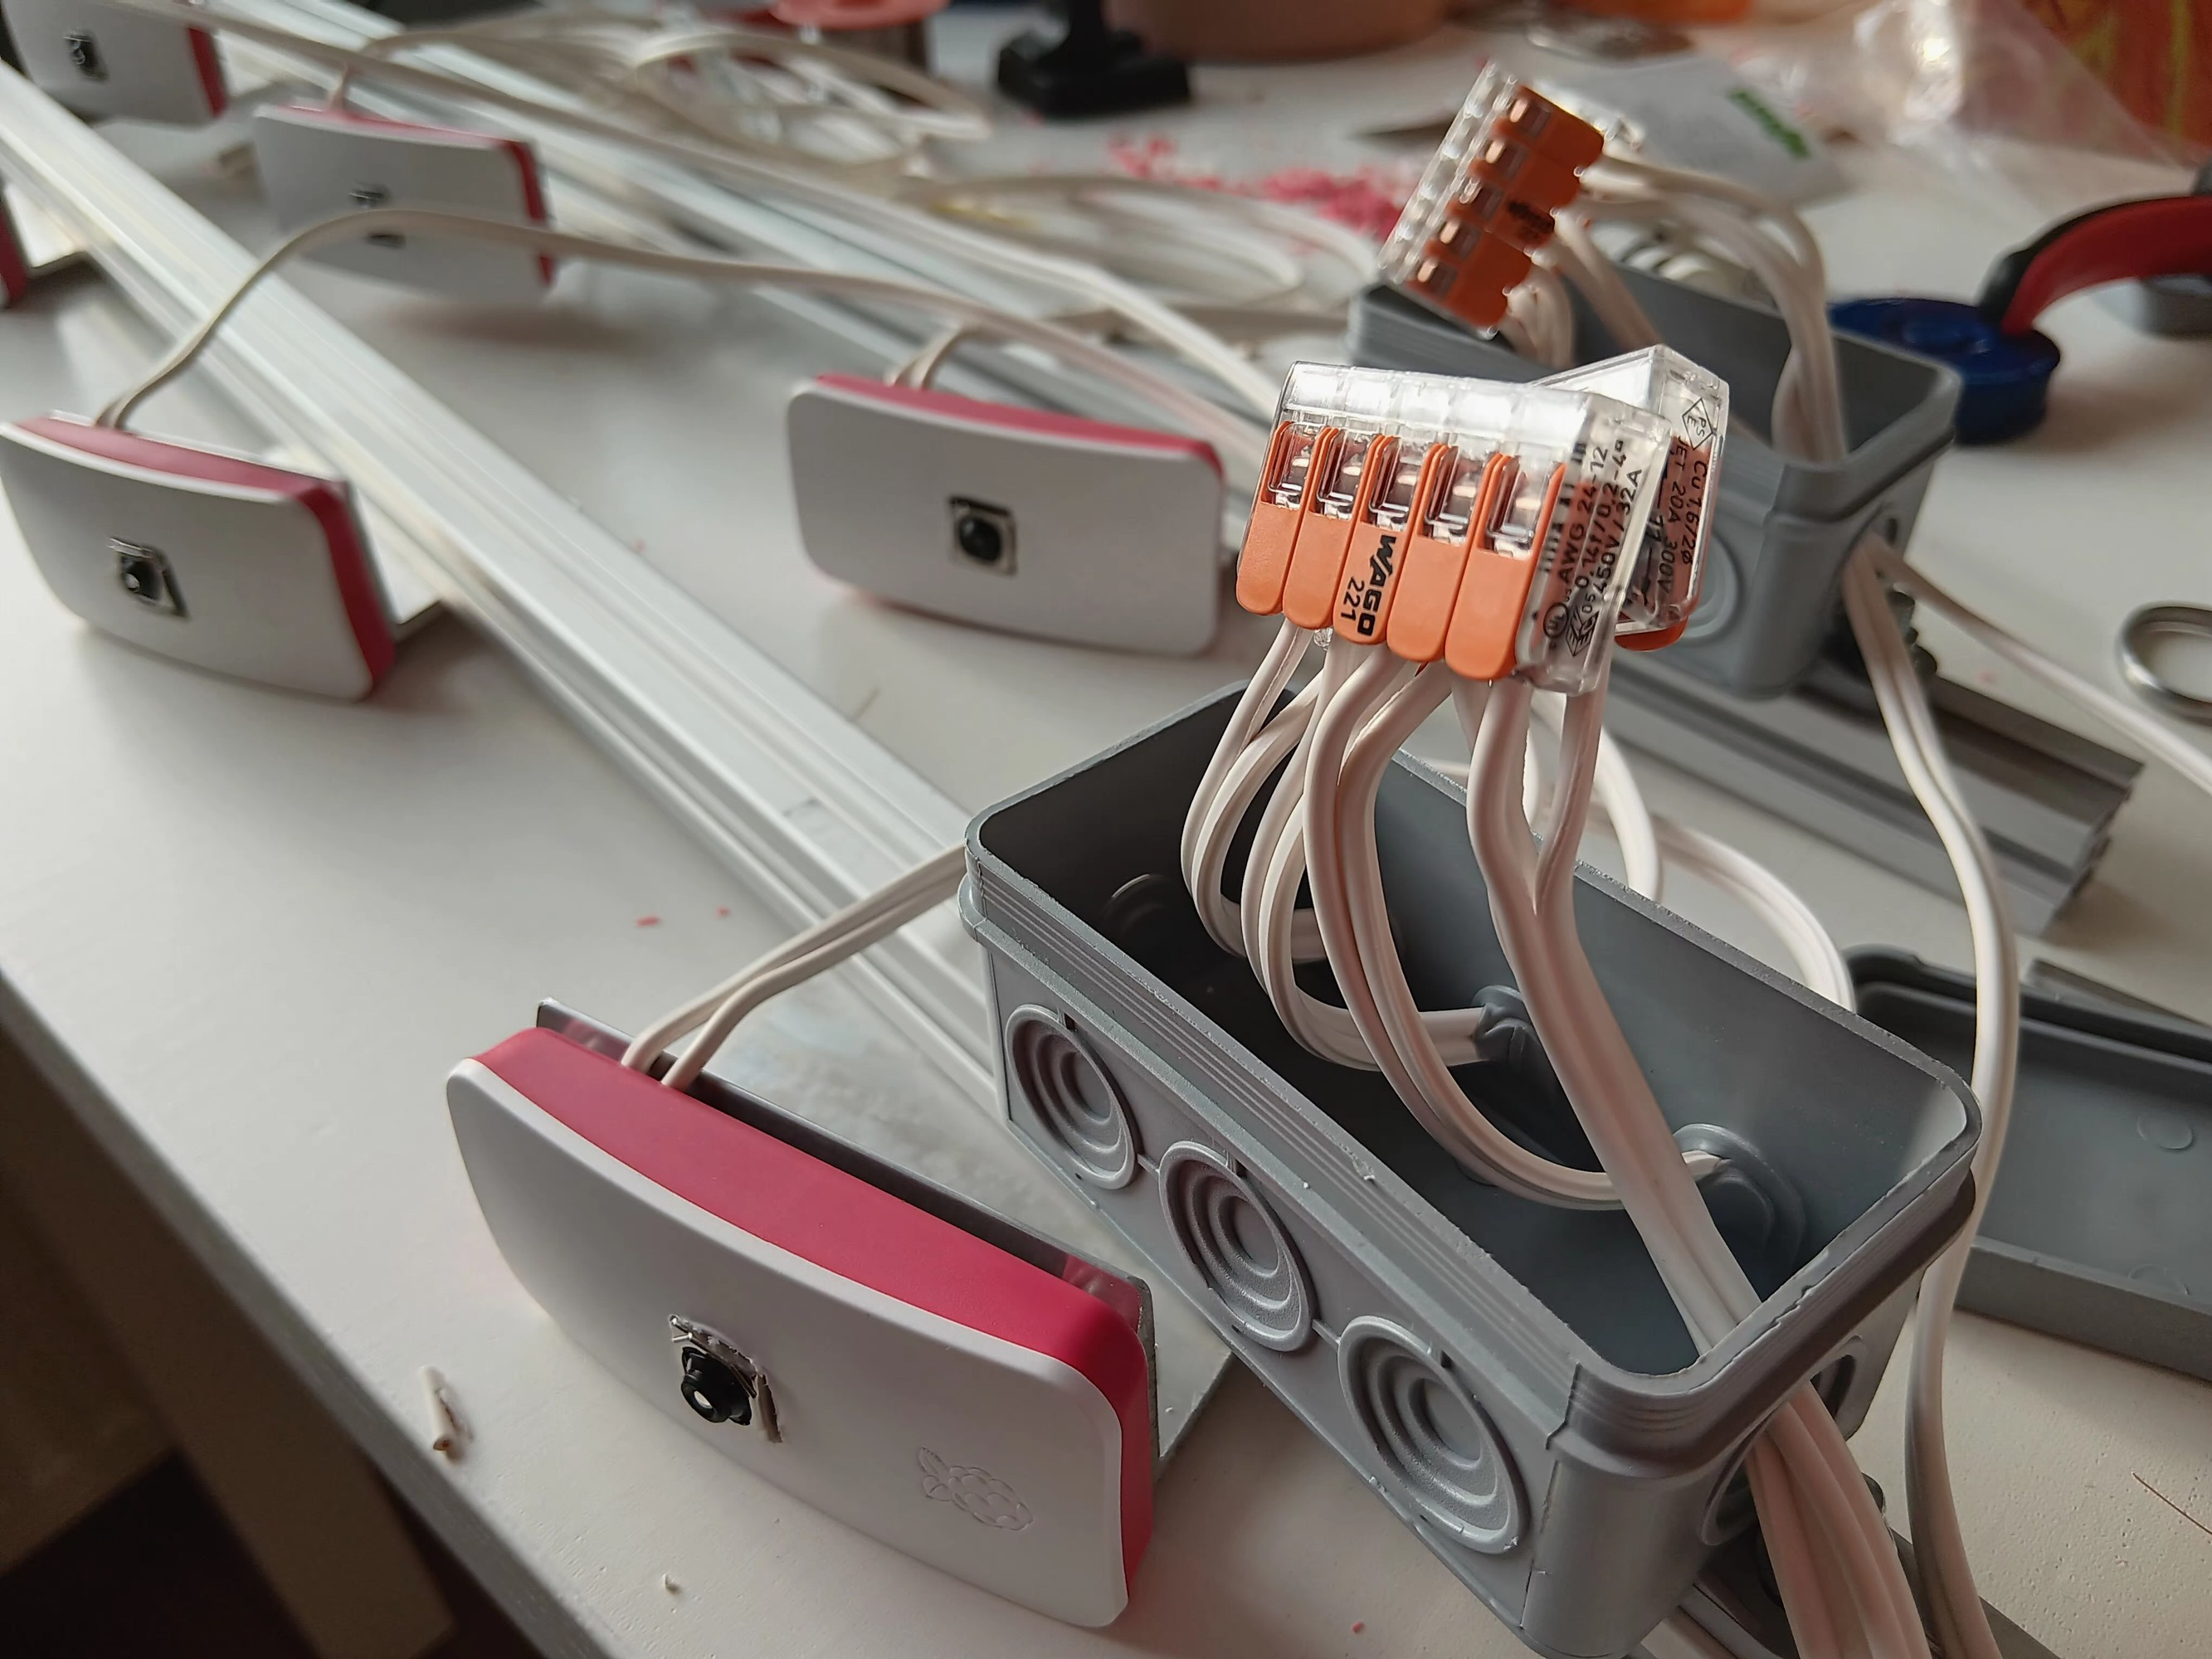
\includegraphics[width=0.7\textwidth]{./img/stromverteilung.jpg}
    \caption{Elektroverteilung zu den einzelnen Raspberry Pi Zero} %Bildunterschrift
    \label{img:stromverteilung} %ID fürs Bild
\end{figure}

Die Raspberry Pi werden mit 5~Volt betrieben. Der Raspberry Pi Zero mit Kamera hatte dabei in Messungen einen maximalen Stromverbrauch von 270~mA aufgezeigt, der Raspberry Pi 4 kann bis zu 1,5~A unter Last verbrauchen. Hieraus ergibt sich ein Gesamtstromverbrauch von maximal rund 8~Ampere. Für den Raspberry Pi 4 wurde ein eigenes Netzteil eingeplant und für die Zero W ein gemeinsames 35 Watt-Netzteil. Versuche zeigten jedoch, dass der Stromverbrauch kurzfristig höher ausfallen konnte, sodass die Zero W, die am meisten von Spannungsabfällen betroffen sind, zum Absturz gebracht wurden, wenn alle Kameras gleichzeitig auslösten. Nachdem die Last auf sicherheitshalber auf zwei weitere Netzteile verteilt wurde, lief das System zuverlässig.

Als Kabelmaterial wurde Klingeldraht mit $0,75~\text{mm}^2$ verwendet. Der relativ hohe Kabelquerschnitt soll für einen geringen Spannungsabfall sorgen. Durch die Verwendung von mehreren Netzteilen ist dieser jedoch nun nicht mehr notwendig. Hier würde sich nun ein geringerer Querschnitt anbieten, auch um eine einfachere Verbindung zu den Raspberry Pi Zero W zu ermöglichen. Diese wurden aufseiten der Zero W verlötet und in den Verteilerdosen mit Federkraftklemmen verbunden (siehe \autoref{img:stromverteilung}).

Die Stromversorgung der Beleuchtung erfolgt über ein 12-V-Netzteil mit $3,5~\text{A}$ Ausgangsleistung. Auch hier wurde Klingeldraht zur Verteilung zwischen den einzelnen Holmen genutzt.

Beim WLAN-Router war ein entsprechendes USB-Netzteil mitgeliefert. Alle Netzteile werden von einer zentralen Steckdosenleiste mit 230V-Netzspannung versorgt. Sie sind alle für eine Wechselspannung zwischen 100 und 240 Volt ausgelegt, sodass mit einem entsprechenden Adapter auch eine Nutzung in anderen Ländern möglich wäre. Die gesamte Energieverteilung ist der \autoref{img:schema_energie} zu entnehmen. Rote Verbindungen stellen hierbei 12-Volt-Leitungen dar, blaue 5-Volt-Leitungen und magentafarbene die 230-Volt-Leitungen. Orange Verbindungen sind Datenleitungen (Steuerleitung LED-Streifen).

\begin{figure}
    \centering
    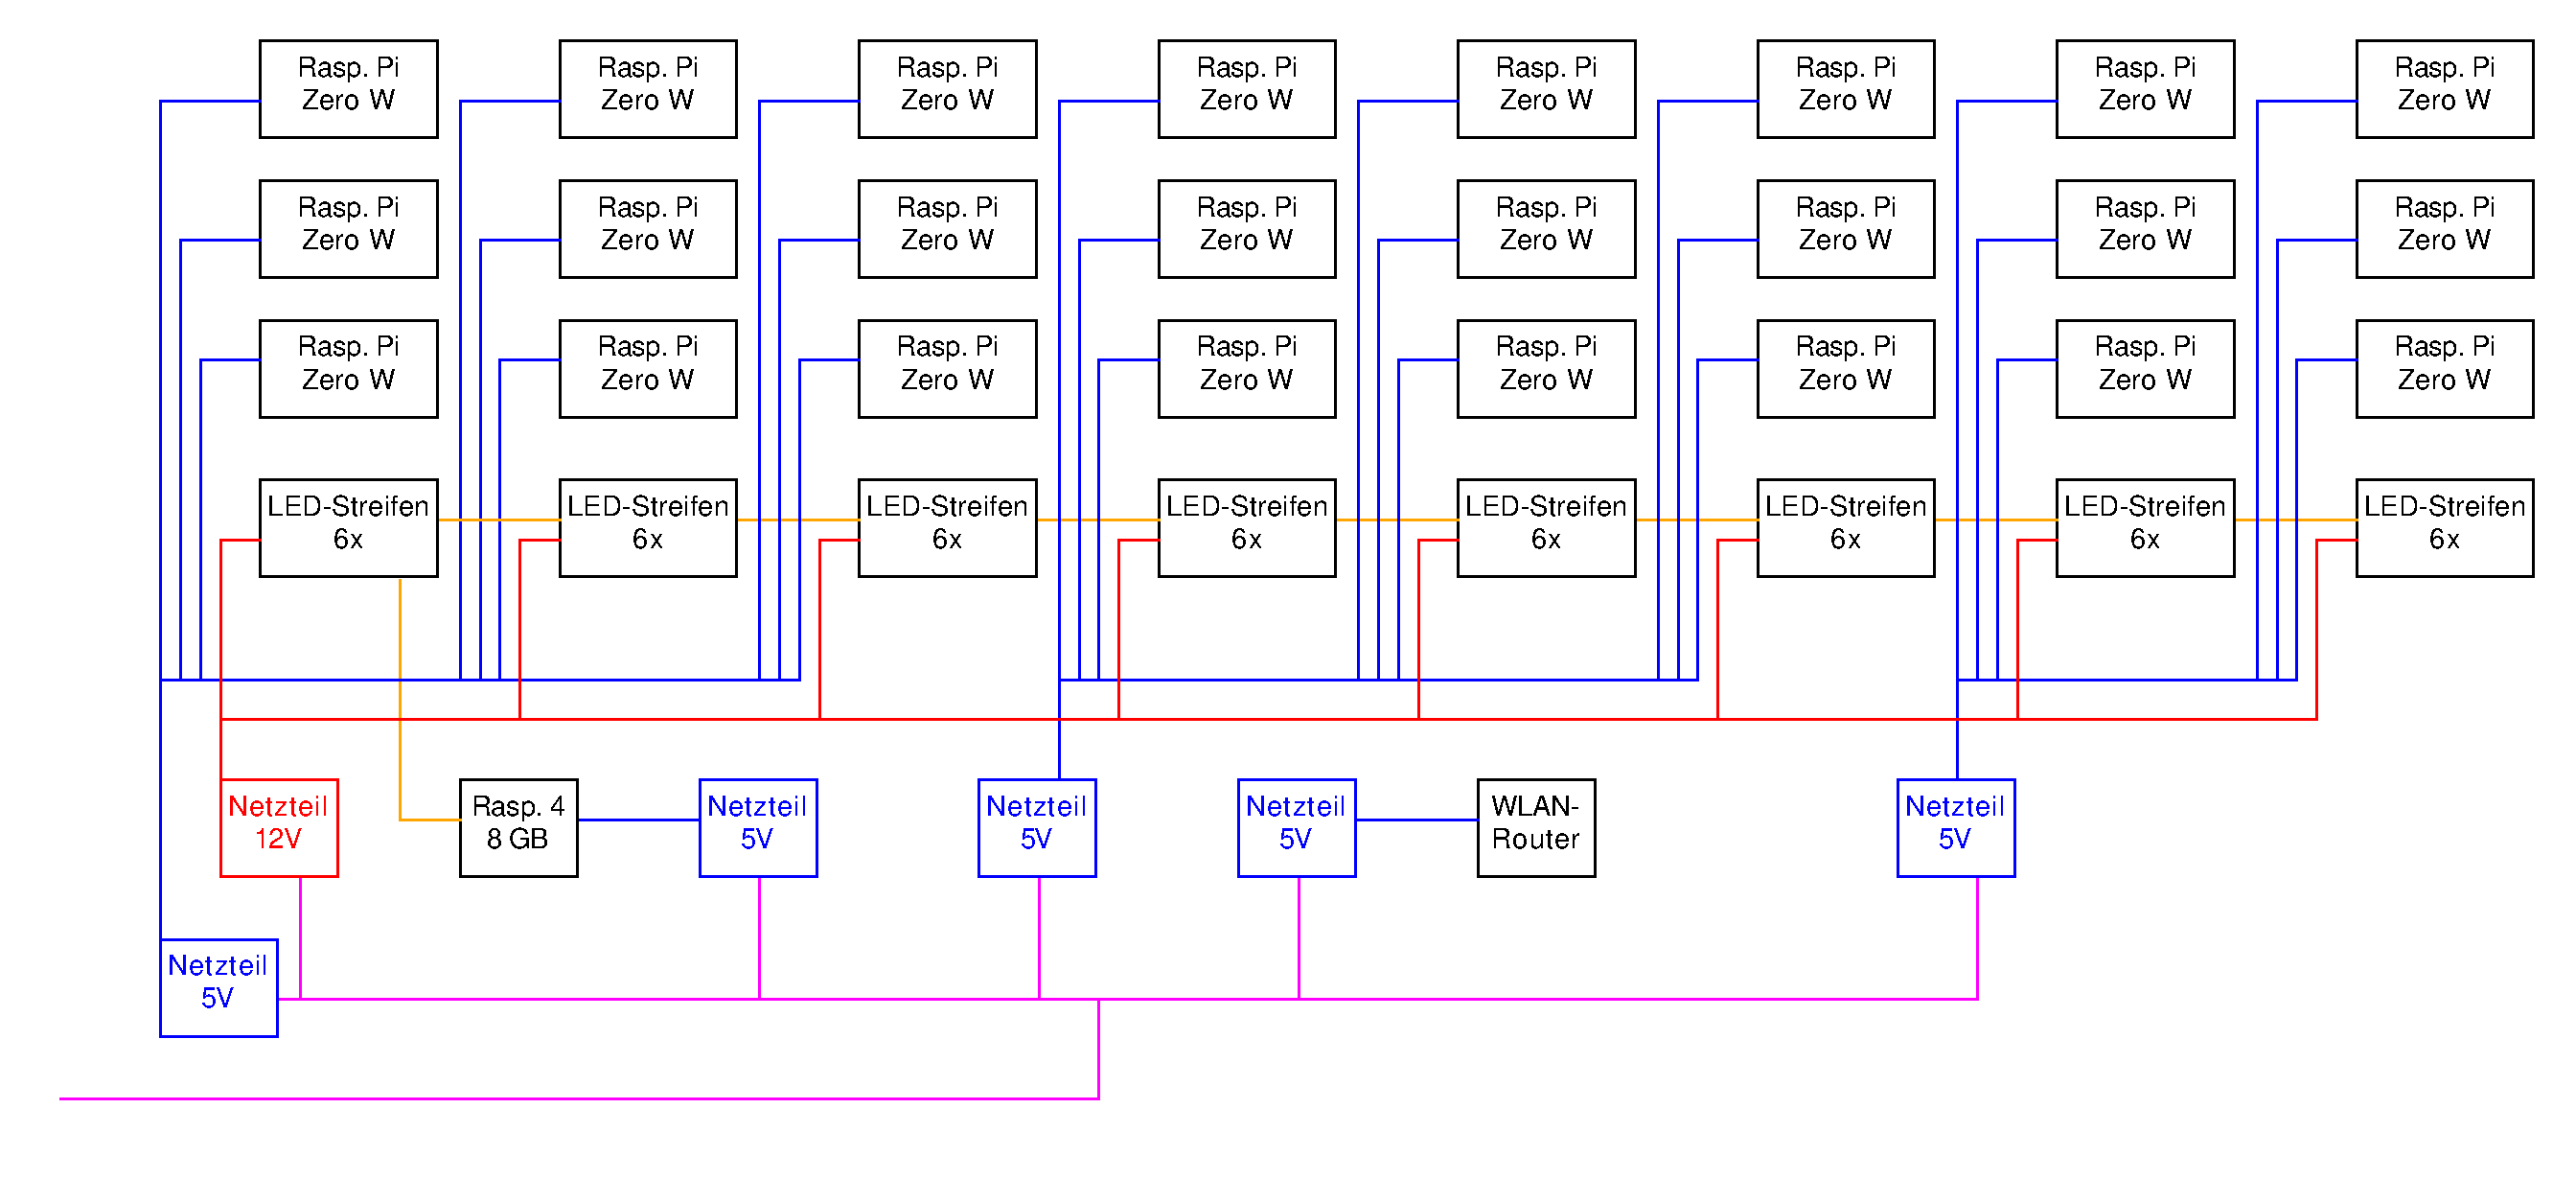
\includegraphics[width=1.\textwidth]{./img/uml/uml_energie.pdf}
    \caption{Schematische Darstellung der Energieversorgung (blau: 5 V; rot: 12 V; magenta: 230 V; orange: Daten)} %Bildunterschrift
    \label{img:schema_energie} %ID fürs Bild
\end{figure}

\section{Kommunikation und Datenübertragung}
Die Kommunikation zwischen den Raspberry Pi erfolgt über WLAN. Vorteil dieser Lösung ist, dass hier keine weiteren Leitungen außer der Stromversorgung zu den einzelnen Raspberry Pi Zero W benötigt wird und es auch möglich wäre, die gleiche Hard- und Software für ein größeres System ohne Änderungen zu nutzen. Nachteilig ist die Verbindungsgeschwindigkeit, gerade im Hinblick auf die Synchronisierung der Kameras. Diese Problematik soll aber durch entsprechende Programmierung der Software möglichst klein gehalten werden.

Als weitere Datenleitungen wird eine Steuerleitung für die LED-Streifen benötigt. Über diese erfolgt die Steuerung der einzelnen LED-Gruppen. Auch hier wurde wieder Klingeldraht verwendet. Sie ist in \autoref{img:schema_energie} in Orange dargestellt.


\biblio
\end{document}